% Instância CMSTP de exemplo: raiz 0 (quadrado) + terminais 1-4 (círculos)
% Arestas sólidas: ligações à raiz; tracejadas: arestas internas
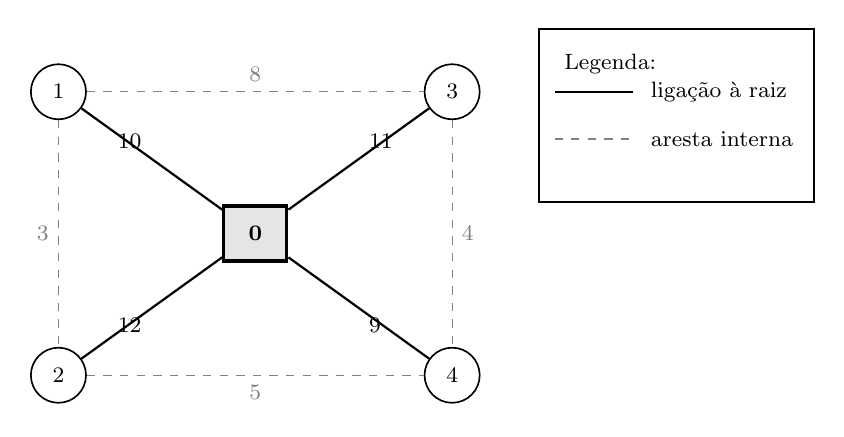
\begin{tikzpicture}
\tikzset{
    >=stealth,
    aresta/.style={-, thick},
    arestaCinza/.style={-, thin, dashed, gray},
    vertice/.style={circle, semithick, draw=black, inner sep=0pt, minimum size=0.7cm},
    raiz/.style={rectangle, very thick, draw=black, fill=gray!20,
                 minimum width=0.8cm, minimum height=0.7cm}
}

% Vértices
\node[raiz]    (v0) at (2.5,2)   {\footnotesize \textbf{0}};
\node[vertice] (v1) at (0,  3.8) {\footnotesize 1};
\node[vertice] (v2) at (0,  0.2) {\footnotesize 2};
\node[vertice] (v3) at (5,  3.8) {\footnotesize 3};
\node[vertice] (v4) at (5,  0.2) {\footnotesize 4};

% Ligações à raiz (custo da aresta)
\draw[aresta] (v0) -- node[above left,  font=\footnotesize] {10} (v1);
\draw[aresta] (v0) -- node[below left,  font=\footnotesize] {12} (v2);
\draw[aresta] (v0) -- node[above right, font=\footnotesize] {11} (v3);
\draw[aresta] (v0) -- node[below right, font=\footnotesize] {9}  (v4);

% Arestas internas
\draw[arestaCinza] (v1) -- node[left,   font=\footnotesize] {3} (v2);
\draw[arestaCinza] (v3) -- node[right,  font=\footnotesize] {4} (v4);
\draw[arestaCinza] (v2) -- node[below,  font=\footnotesize] {5} (v4);
\draw[arestaCinza] (v1) -- node[above,  font=\footnotesize] {8} (v3);

% Legenda
\node[font=\footnotesize, anchor=north west] at (6.3, 4.4) {Legenda:};
\draw[aresta]      (6.3, 3.8) -- (7.3, 3.8);
\node[font=\footnotesize, anchor=west] at (7.4, 3.8) {ligação à raiz};
\draw[arestaCinza] (6.3, 3.2) -- (7.3, 3.2);
\node[font=\footnotesize, anchor=west] at (7.4, 3.2) {aresta interna};
\draw[thick] (6.1,2.4) rectangle (9.6,4.6);
\end{tikzpicture}
